\section{Relational Reasoning in Real-World Tracking}
\label{sec:experiment_real}

\begin{figure}[ht!]
\centering
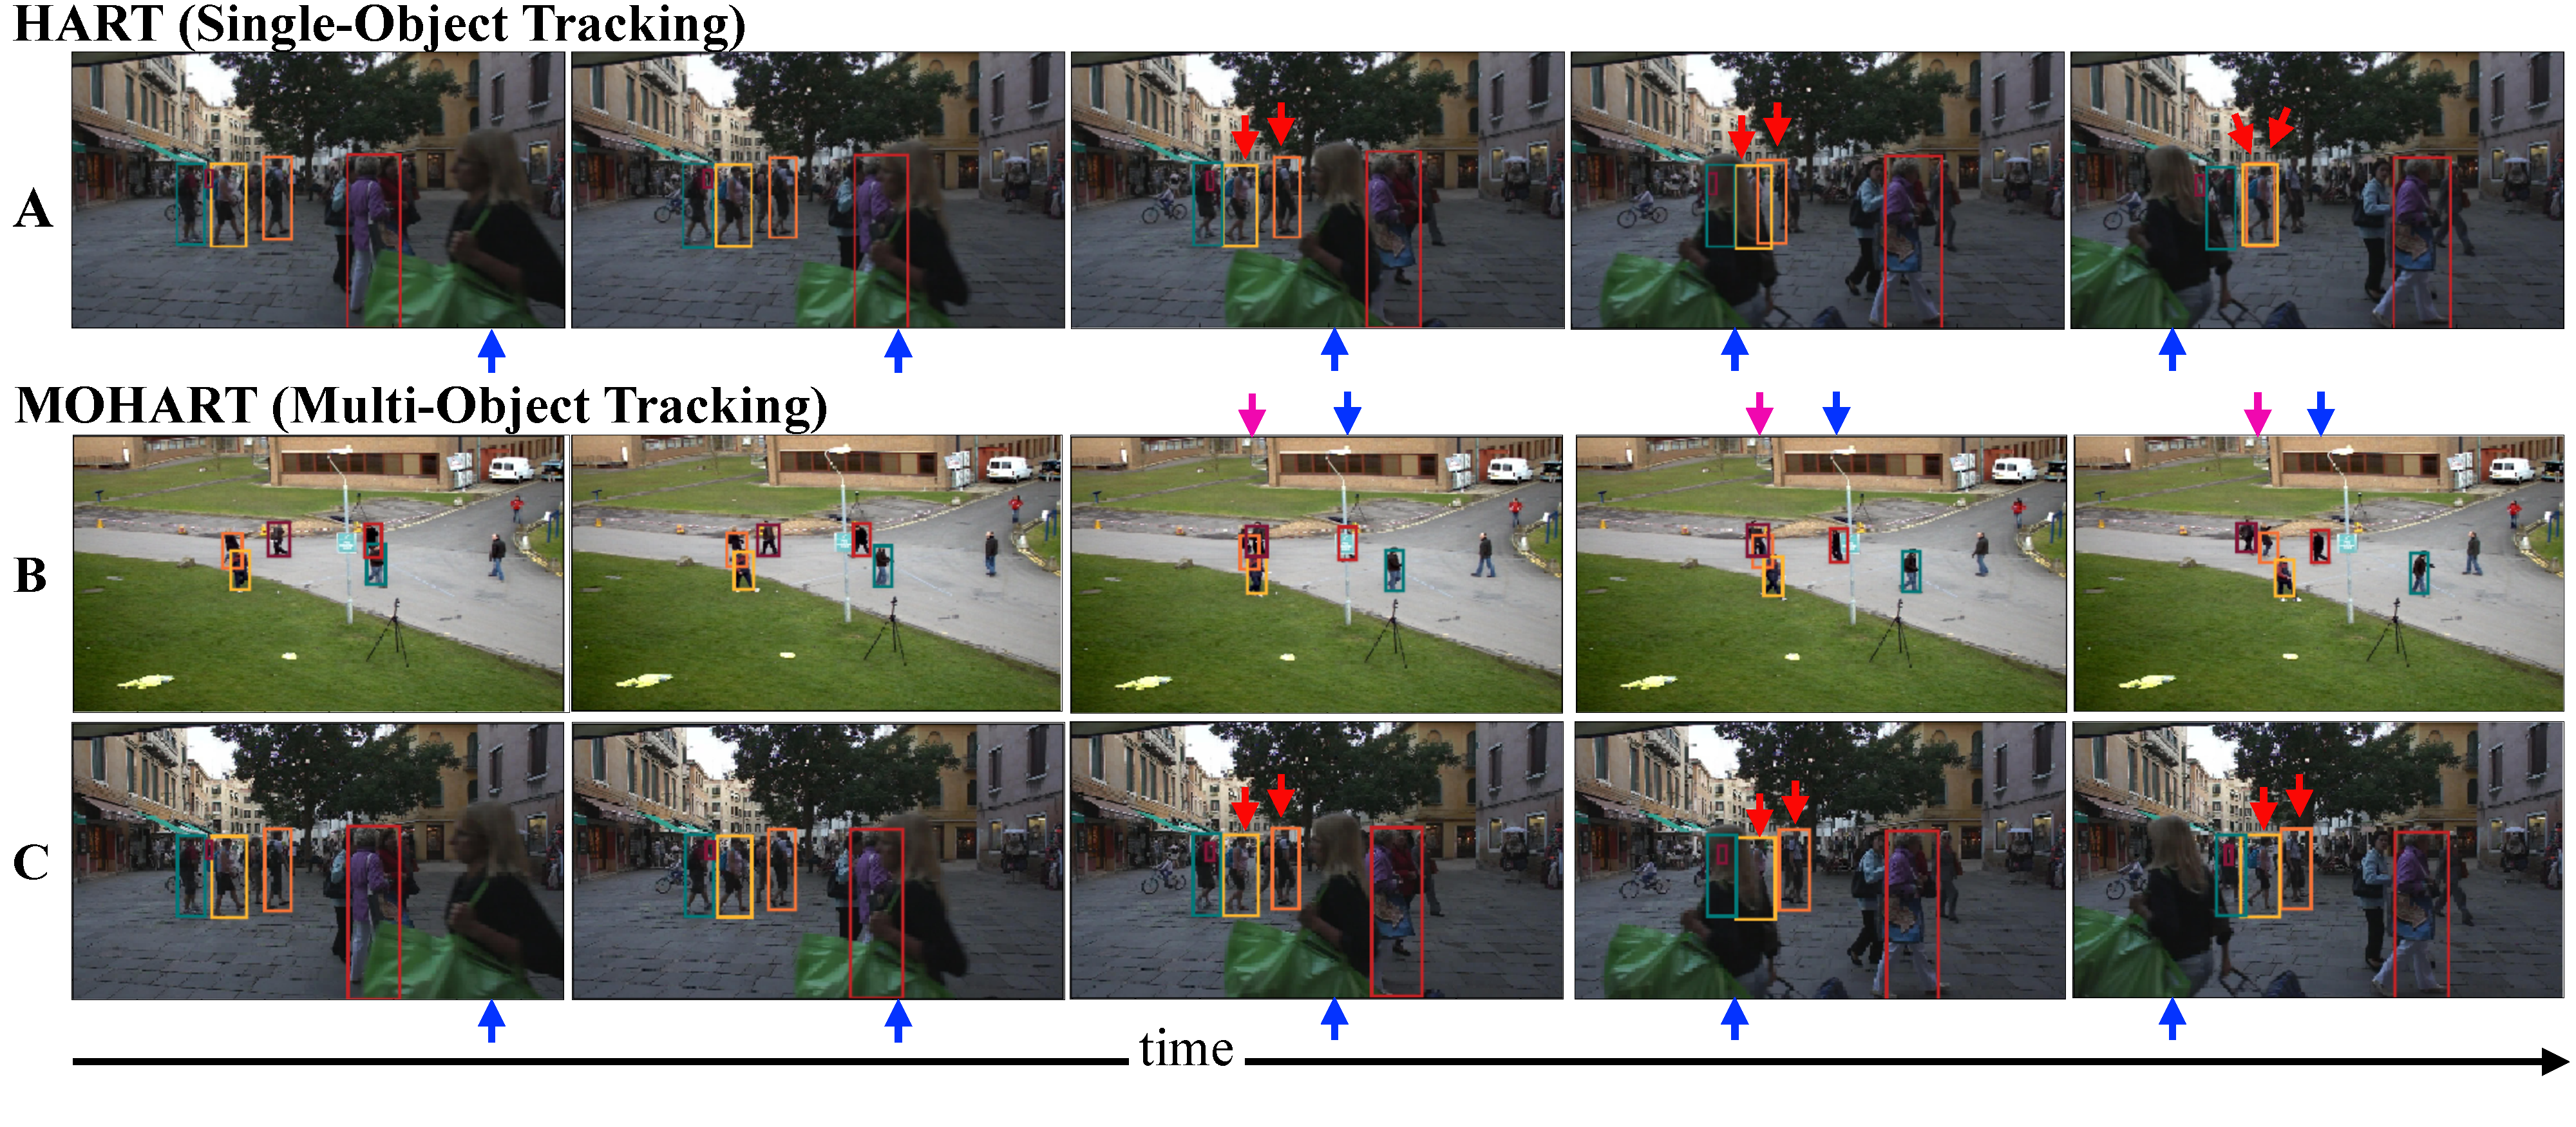
\includegraphics[width=1\textwidth]{figures/MOHART/tracking_qualitative}
\vspace{-8mm}
\caption{Tracking examples of both \textsc{hart} and \textsc{mohart}. Coloured boxes are bounding boxes predicted by the model, arrows point at challenging aspects of the scenes. (A) \& (C): Each person being tracked is temporarily occluded by a woman walking across the scene (blue arrows). \textsc{mohart}, which includes a relational reasoning module, handles this more robustly (compare red arrows).
\vspace{-4mm}}
\label{fig:tracking_and_predicting}
\end{figure}



Having established that \textsc{mohart} is capable of performing complex relational reasoning, we now test the algorithm on three real world datasets and analyse the effects of relational reasoning on performance depending on dataset and task. We find consistent improvements of \textsc{mohart} compared to \textsc{hart} throughout. Relational reasoning yields particularly high gains for scenes with ego-motion, crowded scenes, and simulated faulty sensor inputs.

\subsection{Experimental Details}
\label{sec:exp_details}

We investigate three qualitatively  different datasets: the MOTChallenge dataset \cite{MOT16}, the UA-DETRAC dataset \cite{Wen15}, and the Stanford Drone dataset \cite{DroneDataset}. In order to increase scene dynamics and make the tracking/prediction problems more challenging, we sub-sample some of the high framerate scenes with a stride of two. Training and architecture details are given in \Cref{sec:architecture_details} and \Cref{sec:experimental_details}.
We conduct experiments in three different modes:


\textbf{Tracking.} The model is initialised with the ground truth bounding boxes for a set of objects in the first frame. It then consecutively sees the following frames and predicts the bounding boxes. The sequence length is 30 time steps and the performance is measured as intersection over union (IoU) averaged over the entire sequence excluding the first frame. This algorithm is either applied to the entire dataset or subsets of it to study the influence of certain properties of the data.

\textbf{Camera Blackout.} This simulates unsteady or faulty sensor inputs. The setup is the same as in 
\textit{Tracking}, but sub-sequences images are blacked out. The algorithm is expected to recognise that no new information is available and that it should resort to its internal motion model.

\textbf{Prediction.} Testing \textsc{mohart}'s ability to capture motion patterns, only the first two frames are shown to the model followed by three black frames. IoU is measured seperately for each time step.



\begin{table}[!ht]
  \floatsetup{floatrowsep=qquad, captionskip=4pt}
        \ttabbox%
    {\begin{tabularx}{\textwidth}{l*{5}{>{\raggedleft\arraybackslash}X}}
      \toprule
&                   Entire &            Only &              No  &               Crowded &           Camera \\%[-0.4em]
&                   Dataset &           Ego-Motion &        Ego-Motion &        Scenes &            Blackout \\
      \midrule
\textbf{MOHART} &   \textbf{68.5\%} &   \textbf{66.9\%} &   \textbf{64.7\%} &   \textbf{69.1\%} &   \textbf{63.6\%}  \\[0.1em]
HART &              66.6\% &            64.0\% &            62.9\% &            66.9\% &            60.6\%  \\
\midrule
$\Delta$ &          1.9\% &             2.9\% &             1.8\% &             2.2\% &             3.0\%  \\ 
\bottomrule
      \addlinespace
      \addlinespace
      \addlinespace
      \end{tabularx}}
    {\caption{Tracking performance on the MOTChallenge dataset measured in IoU.}
      \label{tab:results_motc}}
  \begin{floatrow}[2]

      
    \ttabbox%
    {\begin{tabularx}{0.55\textwidth}{l*{3}{>{\raggedleft\arraybackslash}X}}
      \toprule
      & All & Crowded Scenes & Camera Blackout \\
      \midrule
      \textbf{MOHART} & 68.1\% & \textbf{69.5\%} & \textbf{64.2\%}\\
      [0.1em]
      HART & \textbf{68.4\%} & 68.6\% & 53.8\%\\
      \midrule
      $\Delta$ & -0.3\% & 0.9\% & 0.4\%\\
      \bottomrule
      \end{tabularx}}
    {\caption{UA-DETRAC Dataset}
      \label{tab:results_detrac}}
    \hfill%
    \ttabbox%
    {\begin{tabularx}{0.35\textwidth}{r*{3}{>{\raggedleft\arraybackslash}X}}
      \toprule
      All & Camera Blackout & CamBlack Bikes \\
      \midrule
      \textbf{57.3\%} & \textbf{52.6\%} & \textbf{53.3\%} \\
      [0.1em]
      56.1\% & 53.3\% & 50.7\%\\
      \midrule
      1.2\% & 0.7\% & 2.6\%\\
      \bottomrule
      \end{tabularx}}
    {\caption{Stanford Drone Dataset}
      \label{tab:results_stanford}}
  \end{floatrow}
\end{table}%



\subsection{Results and Analysis}


On the MOTChallenge dataset, \textsc{hart} achieves $66.6\%$ intersection over union (see \Cref{tab:results_motc}), which in itself is impressive given the small amount of training data of only 5225 training frames and no pre-training. \textsc{mohart} achieves $68.5\%$ (both numbers are averaged over 5 runs, independent samples $t$-test resulted in $p < 0.0001$). The performance gain increases when only considering ego-motion data. This is readily explained: movements of objects in the image space due to ego-motion scenarios are correlated and can therefore be better understood when combining information from movements of multiple objects, i.e. performing relational reasoning. In another ablation, we filtered for only crowded scenes by requesting five objects to be present for, on average, 90\% of the frames in a sub-sequence. For the MOT-Challenge dataset, this only leads to a minor increase of the performance gain of \textsc{mohart} indicating that the dataset exhibits a sufficient density of objects to learn interactions. The biggest benefit from relational reasoning can be observed in the \textit{camera blackout} experiments (setup explained in \Cref{sec:exp_details}). Both \textsc{hart} and \textsc{mohart} learn to rely on their internal motion models when confronted with black frames and propagate the bounding boxes according to the previous movement of the objects. It is unsurprising that this scenario profits particularly from relational reasoning. Qualitative tracking and \textit{camera blackout} results are shown in \Cref{fig:tracking_and_predicting} and in \Cref{sec:blackout}, respectively.

Tracking performance on the UA-DETRAC dataset only profits from relational reasoning when filtering for crowded scenes (see \Cref{tab:results_detrac}). The fact that the performance of \textsc{mohart} is slightly worse on the vanilla dataset ($\Delta = -0.3\%$) can be explained with more overfitting. As there is no exchange between trackers for each object, each object constitutes an independent training sample.

The Stanford drone dataset (see \Cref{tab:results_stanford}) is qualitatively different to the other two as it is filmed from a top down view. The scenes are more crowded and each object only covers a small number of pixels rendering it a difficult problem for tracking. The dataset was designed for trajectory prediction, a problem setup where an algorithm is typically provided with ground truth tracklets in coordinate space and potentially an image as context information. The task is then to extrapolate these tracklets into the future. The tracking performance profits from relational reasoning more than on the UA-DETRAC dataset but less than on the MOTChallenge dataset. The performance gain on the \textit{camera blackout} experiments are particularly strong when only considering cyclists. 


\begin{figure}
    \centering
    \begin{subfigure}[c]{0.99\linewidth}
        \centering
        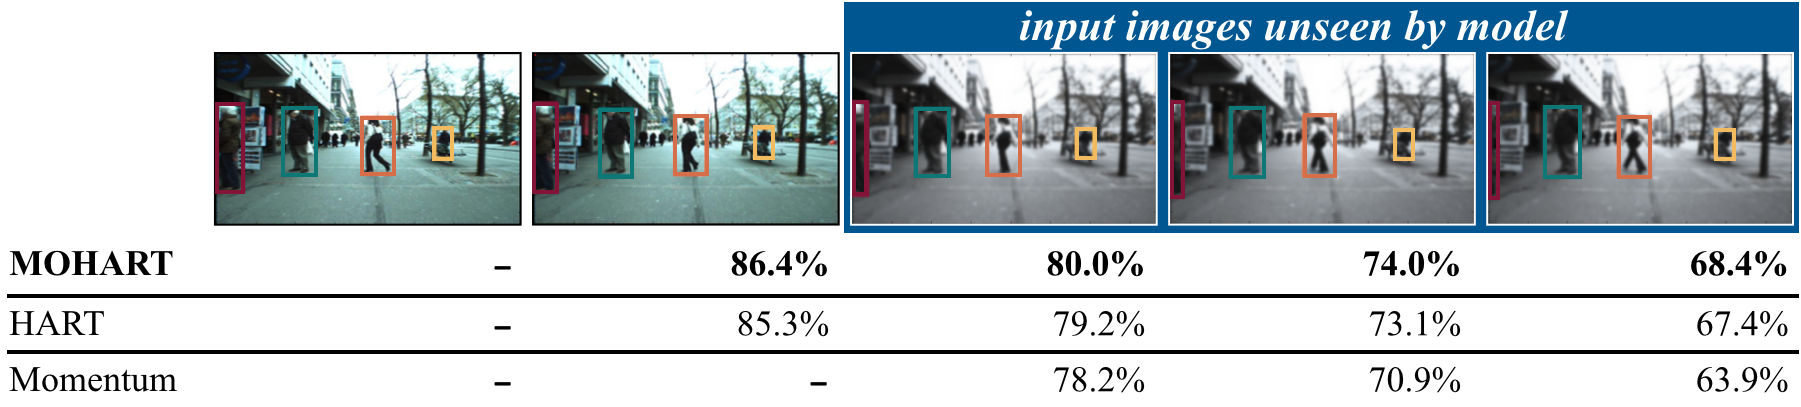
\includegraphics[width=\linewidth]{figures/MOHART/prediction_motc2.png}
        \vspace{-6mm}
        \caption{Prediction results on the MOTChallenge dataset \cite{MOT16}.}
        \label{fig:MOTC_imgs}
    \end{subfigure}
    \vspace{2mm}
    \begin{subfigure}[c]{0.99\linewidth}
        \centering
        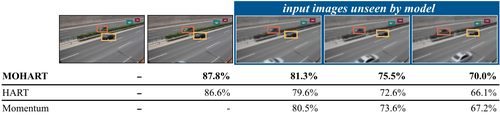
\includegraphics[width=\linewidth]{figures/MOHART/prediction_detrac2.png}
        \vspace{-6mm}
        \caption{Prediction results on the UA-DETRAC dataset (crowded scenes only) \cite{Wen15}.}
        \label{fig:Detrac_quant}
    \vspace{-5mm}
    \end{subfigure}
\caption{Peeking into the future. Only the first two frames are shown to the tracking algorithm followed by three black frames. \textsc{mohart} learns to fall back on its internal motion model when no observation (i.e. only a black frame) is available. The reported IoU scores show the performance for the respective frames 0, 1, 2, and 3 time steps into the future.
\label{fig:prediction}
}
\end{figure}

In the results from the \textit{prediction} experiments (see \Cref{fig:prediction}) \textsc{mohart} consistently outperforms \textsc{hart}. On both datasets, the model outperforms a baseline which uses momentum to linearly extrapolate the bounding boxes from the first two frames. This shows that even from just two frames, the model learns to capture motion models which are more complex than what could be observed from just the bounding boxes (i.e. momentum), suggesting that it uses visual information (\textsc{hart} \& \textsc{mohart}) as well as relational reasoning (\textsc{mohart}). The strong performance gain of \textsc{mohart} compared to \textsc{hart} on the UA-DETRAC dataset, despite the small differences for tracking on this dataset, can be explained as follows: this dataset features little interactions but strong correlations in motion. Hence when only having access to the first two frames, \textsc{mohart} profits from estimating the velocities of multiple cars simultaneously.
